\scanpage{231}
the extension of this group by the said $\Pi_1$ !

What is wrong, one senses it well enough, is
the fact that this equivalence of categories,
is \unsure{1|0}-isotopic\inserted{(i.e. takes into account the $\Pi_0$ of the spaces of homeomorphisms)}, but neglects the
internal \inserted{topological} structure of the topological spaces
\deleted{\unsure{continuous maps} (\illegible{1}} $\mathrm{Homéo}(X,X')$, which one
brutally replaces by their $\Pi_0$ --- neglecting
the homotopy structure of the connected
components, which are (as torsors
under topological groups $\simeq A_{g,\nu}^{\circ}$) homeomorphic
to $A_{g,\nu}^{\circ}$. It is \deleted{\unsure{precisely}} in the
anabelian case, and in that case only,
that this group is $\infty$-connected. In
the abelian case, experience proves that,
the preceding description must be replaced
by Ladegaillerie's in terms \deleted{\illegible{1}}
\unsure{$B_{D^{*}}\longrightarrow B_u$} or \unsure{$\Pi_{D^{*}}\longrightarrow\Pi_u$}, \deleted{\illegible{2}} it
then becomes \inserted{in \unsure{all} cases $\ne$ \unsure{$(0,0)$}} \unsure{$\infty$}-faithful (i.e. takes into account
the $\Pi_i(A_{g,\nu}^{\circ})$). The only case
\margin{\uline{N.B.} There \unsure{is no} \illegible{1} $k$ here --- \illegible{2} \unsure{$T$|$J$} is described \unsure{intrinsically} \unsure{from the structure} of topoi or of groupoids}
\margin{230}

\scanpage{232}
\mspage{116}
entirely refractory (\unsure{and of importance}, it
must be said !) is that of type $0,0$, i.e.
of surfaces homeomorphic to the sphere $S^2$
--- the homotopy type of \deleted{\illegible{1}}
\[
\inserted{A_0^\circ=A_0^+}\deleted{\unsure{A_0^\circ}}
\simeq \mathrm{GP}(1,\mathbb C)\simeq
\underset{(\text{quaternions})}{S^3/\pm1}
\]
and in particular \unsure{its|its} \unsure{$\Pi_i$|$\Pi_1$}, not being at
all well known. To begin with one would have
to \deleted{\unsure{find the}} make explicit the
\unsure{group-category} \inserted{\unsure{$\mathcal G$}}, with invariants $\Pi_0\xrightarrow[\sim]{\chi}\{\pm1\}$ and
$\Pi_1\xrightarrow{\sim}\Pi_1(A_0^\circ)\simeq\pm1$, deduced from \deleted{\unsure{$\mathrm{GP}(1,\mathbb C)$}}\inserted{$A_0$}
by killing the higher homotopy groups
$\Pi_i$ $(i\geq2)$ of $A_0$, or if one prefers,
from the group of conformal automorphisms,
of the Riemann sphere (split extension
of \unsure{$\mathbb Z_2$|$\mathbb Z/2$} by $\mathrm{GP}(1,\mathbb C)$.
The $2$-isotopic $2$-category
of surfaces homeomorphic to \deleted{\unsure{$S^2$}}
\unsure{$\mathrm{GP}(1,\mathbb C)$} is then described by \deleted{that}\inserted{the $2$-groupoid} of
$1$-torsors under the preceding \unsure{group-category}.
\margin{\unsure{We may assume|Observe} that \unsure{$\mathcal G$} \unsure{has only two} objects \unsure{corresponding} to the identity and complex conjugation of the Riemann sphere \unsure{$\widehat{\mathbb C}$|$\overline{\mathbb C}$}, in fact it is \unsure{splittable|split} and even canonically \uline{split} \unsure{!}\ldots}
\margin{231}

\scanpage{233}
\margin{A digression !}
\uline{20} $2$-isotopic description of the category of topological spheres

Here is a way to find a
$1$-isotopic description (and even $2$-isotopic, \unsure{as it happens})
by using a canonical covering \inserted{group}
$\widetilde A_0$ of $A_0$ \deleted{\unsure{of}}, fitting into the exact sequence
\[
(62)\qquad
1\longrightarrow\underset{\substack{\Vert\\\{\pm1\}}}{\mu_2(\mathbb C)}
\longrightarrow\widetilde A_0\longrightarrow A_0\longrightarrow1,
\]
which contains the \deleted{\illegible{1}} corresponding exact sequence
of subgroups
\[
(63)\qquad
1\longrightarrow\mu_2\longrightarrow\widetilde{\mathrm{Sl}}(2,\mathbb C)
\longrightarrow\widetilde{\mathrm{GP}}(1,\mathbb C)\longrightarrow1
\]
where $\widetilde{\mathrm{Sl}}(2,\mathbb C)$ is made up of the $\frac12$-linear \unsure{automorphisms},
of $\mathbb C^2$ (for an unspecified $\mathbb R$-automorphism \inserted{$\rho$},
$\mathrm{id}$ or complex conjugation $\tau$), such that the corresponding
$\rho$-linear automorphism of $\bigwedge^2\mathbb C^2\simeq\mathbb C$
is the identity if $\rho=\mathrm{id}$, and is $\tau:z\longrightarrow\bar z$
if $\rho=\tau$ (i.e., independently \unsure{of the|of the} case, \deleted{\illegible{1} the}\inserted{one considers}
a unimodular vector space $V$ over $\mathbb R$, whence
$V_{\mathbb C}$ over $\mathbb C$, with a restriction of $\bigwedge^2 V_{\mathbb C}$ to $\mathbb R$,
\unsure{whence|thus} a complex conjugation on $\bigwedge^2 V_{\mathbb C}$
--- and a \deleted{\unsure{of the}} basis of $\bigwedge^2 V_{\mathbb C}$ invariant under
this --- and one is interested in the
\unsure{$\rho$|$\mathbb R$}-linear $(\rho\in\mathrm{Aut}_{\mathbb R}\mathbb C)$ \unsure{automorphisms} of $V_{\mathbb C}$ which on
$\bigwedge^2 V_{\mathbb C}$ are $\mathrm{id}$ or complex conjugation \ldots)
\margin{232}

\scanpage{234}
\mspage{117}
$\widetilde{\mathrm{GP}}(1,\mathbb C)$ identifies with the group of conformal \unsure{automorphisms}
\deleted{\illegible{1} \unsure{not here}}
of the Riemann sphere \deleted{\illegible{1}} $\mathbb P^1_{\mathbb C}\simeq\mathbb P^1(\mathbb C^2)$,
\unsure{or} \unsure{automorphisms} of $\mathbb P^1_{\mathbb C}$ as an $\mathbb R$-scheme.
We \unsure{choose here|let act on} $X_0=\mathbb P^1_{\mathbb C}$, \unsure{so that we have}
a canonical inclusion
\[
(64)\qquad \widetilde{\mathrm{GP}}(1,\mathbb C)\longrightarrow A_0
\]
which is (by what precedes (59)) is a
homotopy equivalence. Unless I am mistaken
it follows \inserted{(unless I am mistaken)} that the classification of
extensions of the topological group \inserted{$A_0$} by a group
\unsure{discrete|say} $\mu$ is equivalent, by the restriction
functor, to the category of corresponding
extensions for \deleted{\unsure{$\widetilde A_0$}} $\mathrm{GP}(1,\mathbb C)$, which
makes it possible to construct $\widetilde A_0$, up to unique
isomorphism. This being so, the datum of
a surface \inserted{compact oriented $X$} of genus $0$, which is equivalent
to that of a torsor \unsure{$[\mathrm{Isom}(\mathbb P^1_{\mathbb C},X))$|$(\mathrm{Isom}(\mathbb P^1_{\mathbb C},X))$}
under $A_0$, defines $1^\circ$) the torsor under
$(\pm1)$ deduced from it by $\chi:A_0\longrightarrow\{\pm1\}$
(which is surjective, with kernel $A_0^\circ$) and \unsure{$\varphi$} $2^\circ$) of the
\margin{\uline{N.B.} $\widetilde{\mathrm{GP}}(1,\mathbb C)$ is \unsure{also} the group of \unsure{$\mathbb R$}-linear \unsure{automorphisms} of the \unsure{$\mathbb R$-algebra} $M_2(\mathbb C)$ \deleted{\illegible{3}} (and the \unsure{$\infty$}-isotopic classification of $2$-spheres is therefore equivalent to that of \unsure{simple} algebras of rank $4$ over \deleted{\illegible{1}} a \unsure{not} specified quadratic extension of $\mathbb C$\ldots)}
\margin{233}

\scanpage{235}
groupoid of liftings of this \deleted{\unsure{functor}}\inserted{\unsure{$A_0$}}
torsor to an $\widetilde A_0$-torsor, which is
a connected groupoid ($=$ gerbe) banded by \inserted{the abelian band}
$\underbrace{\mu_2(\mathbb C)=(\pm1)}_{\mu}$,
and in which consequently $\mathrm{Tors}(\mu)$ \inserted{$\simeq\mathrm{Ens}_2$} operates
(it is a $1$-torsor under the group-category
$\mathrm{Tors}(\mu)$). Thus associating to every $X$
the pair \unsure{$(\omega,\mathcal R)$} of the associated $\mu$-torsor $\omega$
(i.e. the $2$-element set of the two orientations of
$X$, or what amounts to the same, the \unsure{module}
of orientations of $X$), plus the \inserted{$\mu$-}groupoid
\unsure{$\mathcal R$}, one finds a $2$-functor from the
$2$-isotopic $2$-category of topological $2$-spheres,
to the $2$-category of pairs \unsure{$(\omega,\mathcal R)$},
and this is an equivalence of
$2$-categories (from this point of view \unsure{one feels}
like saying that it is $3$-faithful,
but since \deleted{\illegible{1}} essential surjectivity
on objects is trivial, the name
$2$-faithful is better, and even (since in
describing it we took care to preserve,
\margin{234}

\scanpage{236}
\mspage{118}
the $\Pi_1$ \inserted{(in addition to the $\Pi_0$)} of the connected components of the \inserted{($A_0$-torsors)}
$\mathrm{Isom}(X_0,X)$, which are $A_0^\circ$-torsors
\unsure{thus} with $\Pi_1$ \unsure{Isomorphic|isomorphic} to $\mu=\{\pm1\}$, it is
even better to call it $1$-faithful ---
but in fact it is even $2$-faithful
(in the corresponding sense) thanks to
the fact that
\diagram{\begin{tikzcd}[ampersand replacement=\&,column sep=2.5em,row sep=1.2em]
(65)\quad\Pi_2(A_0^{\circ})
\& \Pi_2(\mathrm{GP}(1,\mathbb C)) \arrow[l,"\sim"']
\& \Pi_2\bigl(\deleted{\unsure{\mathrm{Sl}(2,\mathbb C)}}\inserted{S^3}/\pm1\bigr)
   \arrow[l,"\sim"']
   \arrow[d,phantom,"{\rotatebox[origin=c]{90}{$\simeq$}}" description]
\\
{} \& {} \& \Pi_2(S^3)=0
\end{tikzcd}}

On the other hand it is not $3$-faithful, for
\[
(66)\qquad \Pi_i(A_0^\circ)\xleftarrow{\sim}\Pi_i(S^3)
\qquad\text{for }i\geq2
\]
and $\Pi_3(S^3)\simeq\mathbb Z\ne0$ hence $\Pi_3(A_0^\circ)\simeq\mathbb Z\ne0$,

We are looking for an $\infty$-isotopic description,
which takes into account the homotopy groups
of all orders (to be determined !) of
$A_0^\circ$ i.e. of $S^3$ (or again, of $\mathrm{Sl}(2,\mathbb C)$,
or of $\mathrm{GP}(1,\mathbb C)$. Up for competition !
\margin{235}

\scanpage{237}
\mspage{119}
But already for the modest description proposed,
\inserted{with pretensions to being} $1$ or $2$-isotopic, for lack of having written
things \unsure{carefully}, I am not too sure whether
the description given is really correct --- I
am a little worried by the fact that I have
not \deleted{\unsure{arranged}}\inserted{imposed} any \deleted{links} relations between the \inserted{$\mu$-}torsor $\omega$,
and the $\mu$-groupoid \unsure{$\mathcal R$}. More generally let
$G$ be a topological group ($\widetilde A_0$, or $\widetilde{\mathrm{GP}}(1,\mathbb C)$),
\figure{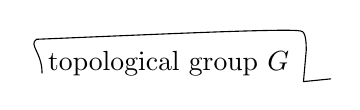
\begin{tikzpicture}[baseline=(phrase.base)]
\node[inner sep=0pt,anchor=base west] (phrase) at (0,0) {topological group $G$};
\draw[line width=0.4pt]
 ([xshift=-2pt,yshift=1pt]phrase.south west)
 .. controls ([xshift=-2pt,yshift=4pt]phrase.west)
          and ([xshift=-7pt,yshift=2pt]phrase.north west)
 .. ([xshift=-4pt,yshift=4pt]phrase.north west)
 .. controls ([yshift=6pt]phrase.north)
          and ([yshift=8pt]phrase.north east)
 .. ([xshift=4pt,yshift=7pt]phrase.north east)
 .. controls ([xshift=6pt,yshift=7pt]phrase.north east)
          and ([xshift=6pt,yshift=2pt]phrase.north east)
 .. ([xshift=6pt]phrase.north east)
 -- ([xshift=5pt,yshift=-2pt]phrase.south east)
 -- ([xshift=15pt,yshift=-1pt]phrase.south east);
\end{tikzpicture}}
such that \deleted{\unsure{$\widetilde A_0^\circ$}}\inserted{$G^\circ$} is simply connected; \deleted{let}
\deleted{\unsure{set} $\mu=\mathrm{Centre}(\unsure{\widetilde A_0^\circ})$}
\[
(67)\qquad\Pi_1(G^\circ)=0
\]
let
\[
(68)\qquad \mu=\mathrm{Centre}(G^\circ),\qquad\Gamma=G/G^\circ
\]
\margin{we assume $\mu$ discrete (thus $G^\circ$ identifies with the universal covering group of $G^\circ/\mu=\mathcal H^\circ$ (if $\mathcal H=G/\mu$))}
then the topological group extension $G$
of $\Gamma$ by $G^\circ$ defines
\[
(69)\qquad\Gamma\longrightarrow\mathrm{Aut\,ext}(G^\circ)
\qquad(\longrightarrow\mathrm{Aut}(\mu).)
\]
and the set of classes of extensions corresponding
to a given \inserted{outer} operation of $\Gamma$ on $G^\circ$
is in a natural way a torsor under
$H^2(\Gamma,\mu)$ (if it is not empty, which \unsure{is|we have} excluded
by the starting hypothesis, starting from $G$\ldots)
\margin{236}

\scanpage{238}
This category of extensions is moreover equivalent
\deleted{It \unsure{corresponds}}
to that of splittings of a certain
group-category defined by Sinh \inserted{via $(69)$}, whose $\Pi_0$ and
$\Pi_1$ are respectively $\deleted{\unsure{\Pi_0}}\Gamma$ and $\mu$ --- which
is \inserted{thus} here split by the datum of the extension
$G$. (In the case that interests us,
$\Gamma\simeq\mu\simeq\{\pm1\}$, and
this extension is even split, and corresponds
to an operation of order $2$ of $\Gamma$ on $G^\circ$,
which I very much doubt is an inner automorphism.
In fact, I have the impression that in the
two cases we are dealing with ($\widetilde{\mathrm{GP}}(1,\mathbb C)$ and
$\widetilde A_0$) that $(69)$ is an \uline{isomorphism}
$\Gamma=\{\pm1\}\xrightarrow{\sim}\mathrm{Autext}(G^\circ$

This being so, the datum of a torsor under
$\mathcal H=G/\mu$ defines $1^\circ$) a torsor under $\Gamma$,
$\mathcal H\longrightarrow\Gamma\simeq\mathcal H/\mathcal H^\circ$; $2^\circ$) the groupoid of
liftings of liftings of this torsor
to a torsor under $G$, which is a
\inserted{connected} $\mu$-groupoid (on which $\mu$ operates).
\margin{We assume that $\Gamma$ operates \uline{trivially} on $\mu$ i.e. $\mu\subset\mathrm{Centre}(G)$}

If we \deleted{\unsure{exp}} take this up again in terms of bundles
over a base space $S$ we find
\margin{237}

\scanpage{239}
\mspage{120}
again on $S$ (for every topological $\mathcal H_S$-torsor)
a pair $(\omega,\unsure{\mathcal R|R})$ of a $\Gamma$-torsor, and of
a $\mu$-gerbe on $S$, which are described (up to \unsure{isomorphism}
\inserted{\illegible{1} \unsure{equivalence}}
\unsure{up to equivalence|and equivalence}) by $H^1(S,\Gamma)$ and $H^2(S,\mu)$
respectively. We would like to isolate
conditions \inserted{on $G$ and on $S$} for the map
\[
(70)\qquad H^1(S,\mathcal H)\longrightarrow H^1(S,\Gamma)\times H^2(S,\mu)
\]
to be bijective.
\margin{\uline{N.B.} $\omega$ does not depend on the choice of the extension \unsure{$\widetilde G$} of $\mathcal H$ by \unsure{$\mathfrak z$|$\zeta$}${}\simeq\Pi_1(\mathcal H^\circ)$; \unsure{on the other hand} $\mathcal R$ depends on it (and one \unsure{would have to} see how)}

Injectivity : If the image \inserted{of a $\zeta\in H^1(S,\mathcal H)$,}
in $H^2(S,\mu)$ is zero,
the element of $H^1(S,\mathcal H)$ lifts to an element $\widetilde\zeta$
of $H^1(S,\widetilde{\mathcal H}=G)$; \unsure{whose} image in $H^1(S,\Gamma)$
\unsure{under} $G\longrightarrow\Gamma$ is the same as that of $\zeta$, so if
it is trivial, one sees that $\widetilde\zeta$ comes from
a $\widetilde\zeta_0\in H^1(S,G^\circ)$. If we know that
$H^1(S,G^\circ)=(1)$, we win. By the
sledgehammers of homotopy, it works
if $\exists n\in\mathbb N$ with
\[
\Pi_i(G^\circ)=0\quad\text{if}\quad i\leq n
\]
\inserted{(thus $\Pi_i(B_{G^\circ})=0$ if $i\leq n+1$)}
\deleted{$\Pi_i(S)=0$ if $i>n+1$}
\deleted{$\dim S\leq n+1$}
$S$ a CW-complex of dimension $\leq n+1$
\margin{in the case we are dealing with, one can take $n=2$}

For surjectivity, note that \unsure{for|first} an
\margin{238}

\scanpage{240}
element of $H^2(S,\mu)$, the obstruction to its
lifting to an element \inserted{$\zeta$} of $H^1(S,\mathcal H)$ is
in $H^2(S,G)$ [by the associated exact sequence
of \unsure{cohomology} : $1\longrightarrow\mu_S\longrightarrow G_S\longrightarrow\mathcal H_S\longrightarrow1$]
one must express that a certain \deleted{\illegible{1}} gerbe
banded by $G_S$ is neutral --- brr!. But
let us rather start from the element \inserted{\unsure{$\omega$|$\widetilde\zeta$}} of $H^1(S,\Gamma)$,
if the extension of $\Gamma$ by \deleted{\unsure{$G^\circ$}}$\mathcal H^\circ$ is split, then
one can find a $\zeta_0\in H^1(S,\mathcal H_S)$ which
gives rise to \unsure{$\omega$}. It has a certain
obstruction $\rho_0$ in $H^2(S,\mu)$, and it is a matter
of correcting $\zeta_0$ to $\zeta$, \inserted{in} such a way that
the obstruction becomes the given $\rho\in H^2(S,\mu)$.
\deleted{We have at our disposal} \inserted{Using $\zeta_0$} to twist $\mathcal H_S$ into
$\mathcal H'_S$, and (via the operation of $\mathcal H_S$ \inserted{$=G_S/\mu_S$} on $G_S$,
taking into account that $\mu_S\subset\mathrm{centre}\,G_S$) to
twist $G_S$ also \inserted{into $G'_S$}, whence
\[
1\longrightarrow\mu\longrightarrow G'_S\longrightarrow\mathcal H'_S\longrightarrow1
\]
one finds that the $\zeta$ having the same image in $H^1(S,\Gamma)$
\margin{239}
